\appendix

\section{Bias bound for a mismatched sampling distribution}
\label{app:bias}

For any sampler law $q$, the sampled and variational energies (Sec.~\ref{sec:validation}) differ by
\begin{equation}
\widetilde E_q-E_\theta=\sum_v[q(v)-\pi_\theta(v)]\Eloc(v),
\label{eq:bias}
\end{equation}
so that for finite local energies,
\begin{equation}
|\widetilde E_q-E_\theta|\le[\max_v\Eloc(v)-\min_v\Eloc(v)]\,\DTV(q,\pi_\theta).
\label{eq:biasbound}
\end{equation}
A one-spin example saturates this bound and shows it can be numerically large: for $H=-\sigma^x$, $\pi=(0.99,0.01)$, $\psi=\sqrt\pi$, the variational energy is $E_\theta=-2\sqrt{0.99\times0.01}\approx-0.199$, while a sampler with $q=(0,1)$ gives $\widetilde E_q\approx-9.950$ -- far below $E_0=-1$, without contradicting the variational principle, which bounds $E_\theta$, not $\widetilde E_q$. This is why Sec.~\ref{sec:validation} insists on an independently sampled or exactly enumerated $E_\theta$ rather than the training-time $\widetilde E_q$: a small logged $\widetilde E_q-E_0$ does not bound $E_\theta-E_0$ unless $\DTV(q,\pi_\theta)$ is separately controlled.

\section{Repository audit: what code the placeholders in this paper require}
\label{sec:code-gaps}

Table~\ref{tab:codegaps} summarizes an audit of the implementation repository against the eight capabilities this paper's placeholders depend on. ``Present'' means the capability exists and is used in the current pipeline; ``partial'' means related code exists but does not do what is needed; ``absent'' means no such code was found. File paths and line numbers are current as of the audited checkout and should be re-verified against the commit actually used for any figure regenerated from this table.

\begin{table*}[t]
\caption{Code-gap inventory for the placeholders in Secs.~\ref{sec:thermometry}--\ref{sec:resources}. Repository root: \texttt{adiabatic-boltzmann}.}
\label{tab:codegaps}
\begin{ruledtabular}
\begin{tabular}{lp{0.1\textwidth}p{0.55\textwidth}}
Item & Status & Evidence \\
\hline
T1. Conditional-MLE thermometry (Sec.~\ref{sec:cem-mle}) & Absent & \texttt{src/encoder.py:206--219}, \texttt{estimate\_beta\_eff\_cem}, implements only the pooled least-squares objective Eq.~\eqref{eq:cem-ls} via \texttt{scipy.optimize.minimize\_scalar}. No score-equation (Eq.~\eqref{eq:score}) solver exists anywhere in \texttt{src/} or \texttt{scripts/}. \\
T2. Independent frozen-checkpoint evaluator (Sec.~\ref{sec:protocol}) & Partial & \texttt{scripts/exper/exact\_ansatz\_floor.py} performs exact-enumeration \emph{training} (not evaluation of an already-trained, frozen checkpoint with an independent RNG stream); \texttt{scripts/validation/fill\_reference\_energies.py} only caches exact ground-state energies for computing error, not ansatz evaluation. No \texttt{evaluate\_checkpoint}-type script exists; the training-log rolling-mean energy remains the only per-run energy readout used downstream (e.g.\ \texttt{scripts/viz/plot\_ttc.py}). \\
T3. Survival-corrected $\mathrm{TTE}_{99}$ (Sec.~\ref{sec:tte-issue}) & Absent & \texttt{scripts/viz/paper\_figures.py:148--174}, \texttt{tte99\_from\_validated()}, implements exactly Eq.~\eqref{eq:tte99} (median successful time $\times$ retry factor from $p$); no Kaplan--Meier, right-censoring, or fixed-cutoff-$\tau$ formulation is present. \\
T4. Multi-$(\epsilon,h)$ sweep (Sec.~\ref{sec:eps-h}) & Partial & \texttt{fig\_tte\_vs\_h\_n16()} in \texttt{scripts/viz/paper\_figures.py:1469--1541} sweeps $h\in\{0.5,\dots,1.5\}$ at fixed $\epsilon=0.1$, $N=16$, but is defined and never called from the script's entry point. No script sweeps $\epsilon$; every figure function hardcodes one value ($0.1$ or, for unrelated ITE figures, $0.01$). \\
T5. QPU hardware-resource telemetry (Sec.~\ref{sec:hw-resources}) & Absent & The D-Wave sampling paths in \texttt{src/sampler.py} (e.g.\ lines $\approx$1478, $\approx$1588) read only \texttt{info["timing"]["qpu\_access\_time"]}. A repository-wide search for \texttt{chain\_break\_fraction}, \texttt{broken\_chain}, \texttt{num\_qubits}, \texttt{embedding\_success} returns no hits outside third-party packages. \\
T6. End-to-end vs.\ device timing (Sec.~\ref{sec:resources}) & Partial & \texttt{src/encoder.py:557} forms \texttt{total\_sampling\_time\_s = sample\_time\_s + cem\_time} (device time plus thermometry overhead only); \texttt{wall\_time\_s} is recorded in some pipelines (\texttt{scripts/hparam/hparam\_optuna.py}, \texttt{scripts/ite/ite\_run.py}, \texttt{scripts/j1j2/j1j2\_convergence\_median.py}) but is not decomposed into transfer/embedding/decoding/network components. \\
T7. FPGA algorithm documentation and fidelity test (Sec.~\ref{sec:fpga}) & Partial & \texttt{FPGASampler} in \texttt{src/sampler.py:581--892} documents I/O and configuration and, at lines $\approx$858--865/891--909, the uniform-subsampling rule from 1024 replicas to $\sim\!200$ SR samples (with a bias-avoidance rationale in comments). The transition/update rule and stationary distribution are not documented in this repository -- they live in the external, non-vendored \texttt{VeloxQFPGA} Julia package. No bitstream/toolchain version is pinned (\texttt{FPGA\_BITSTREAM} env var, blank by default); no sample-independence test; no $\DTV$-style fidelity test (\texttt{scripts/dtv/} has no FPGA-referencing file). \\
T8. Measured (not modeled) FPGA/GPU energy (Sec.~\ref{sec:resources}) & Partial & GPU energy is genuinely measured: \texttt{src/energy.py}'s \texttt{GPUEnergyMeter} polls \texttt{nvidia-smi --query-gpu=power.draw} and trapezoidally integrates over marked active windows, without idle-baseline subtraction. FPGA energy is a hardcoded constant: \texttt{scripts/viz/plot\_ite.py:82--86} and \texttt{scripts/viz/paper\_figures.py:1348} both set \texttt{ASSUMED\_POWER\_W\{"fpga/fpga": 45.0\}} $\times$ device time. QPU energy is correctly not estimated at all. \\
\end{tabular}
\end{ruledtabular}
\end{table*}

Items T1--T4 are, in order, the estimator this paper is centrally about, the validation step the evaluation called the single most important repair, the statistic underlying the corrected headline claim of Sec.~\ref{sec:headline}, and the sweep needed to know whether that claim generalizes; they should be prioritized in that order. T5--T8 support Sec.~\ref{sec:resources}'s resource accounting and are independent of the thermometry result itself.

\section{Sparse hardware-native RBMs: a resource note}
\label{app:sparse}

At $N=M=16$, $h=1$ ($E_0=-20.4045944748$), exact-expectation training at 3000 iterations improves several sparse masks substantially over 300 iterations (e.g.\ the $0.808594$-removed mask: median error per spin $0.06341\to0.02162$), while the native hardware mask and the sparsest mask change little. At matched (300) iterations, all three classical samplers tested have larger median error than exact expectations on every shared mask. Figure~\ref{fig:sparse} reproduces both comparisons.

\begin{figure}[h]
\centering
\panel{.48}{\textbf{(a)}\\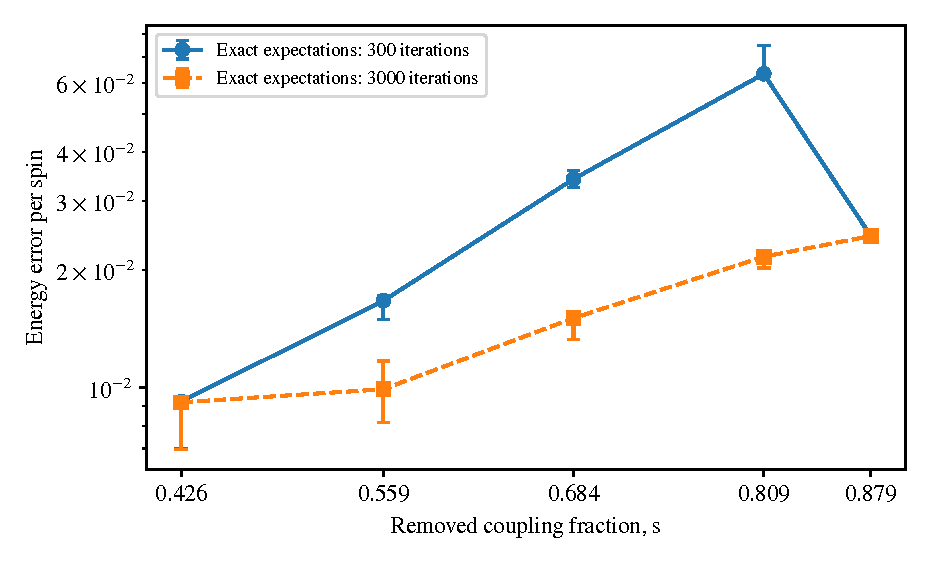
\includegraphics[width=\linewidth]{figures/sparsity_exact_budget.pdf}}\hfill
\panel{.48}{\textbf{(b)}\\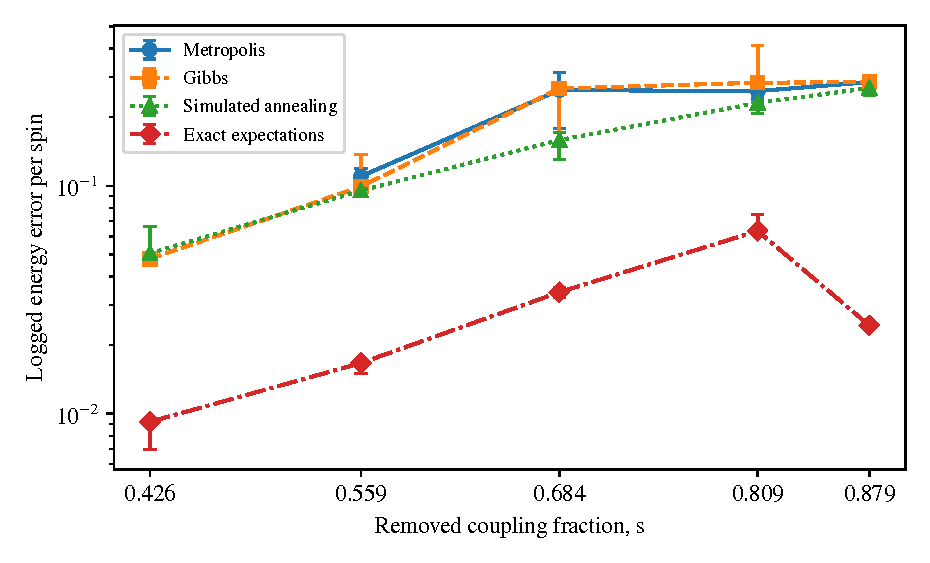
\includegraphics[width=\linewidth]{figures/sparsity_matched_iterations.pdf}}
\caption{(a) Exact-expectation training at 300 vs.\ 3000 iterations across sparsity masks. (b) Matched-iteration (300) comparison of exact expectations against three classical samplers. Five seeds per point; markers are medians, bars span first/third quartiles.}
\label{fig:sparse}
\end{figure}

For any mask $B$, $E_{\mathrm{trained}}\ge E_B^*\ge E_0$, so a favorable exact-expectation result is an achieved upper bound on the best attainable error, not a certified capacity floor -- longer optimization already changes several of these numbers by more than a factor of two. We do not generalize this ablation beyond the tested masks: it shows the tested hardware-derived masks are poor for the tested RBM/TFIM configuration, not that sparse or hardware-native neural quantum states are unsuitable in general.

\section{Simultaneous embeddings: a reliability note}
\label{app:parallel}

Pooling $C$ simultaneously embedded logical copies over $R$ reads returns $CR$ configurations but not necessarily $CR$ independent ones, since shared programming or device fluctuations can correlate copies. In the recorded campaign (one, three, and five copies, three seeds each), four of nine training runs diverge, including two of the three five-copy runs (Fig.~\ref{fig:parallel}). Selecting only converged trajectories would overstate reliability; with three seeds per configuration, this campaign cannot establish a dependable reduction in time-to-validated-state, only that the mechanism is worth a larger study with an explicit per-copy distribution check before pooling.

\begin{figure}[h]
\centering
\panel{.47}{\textbf{(a)}\\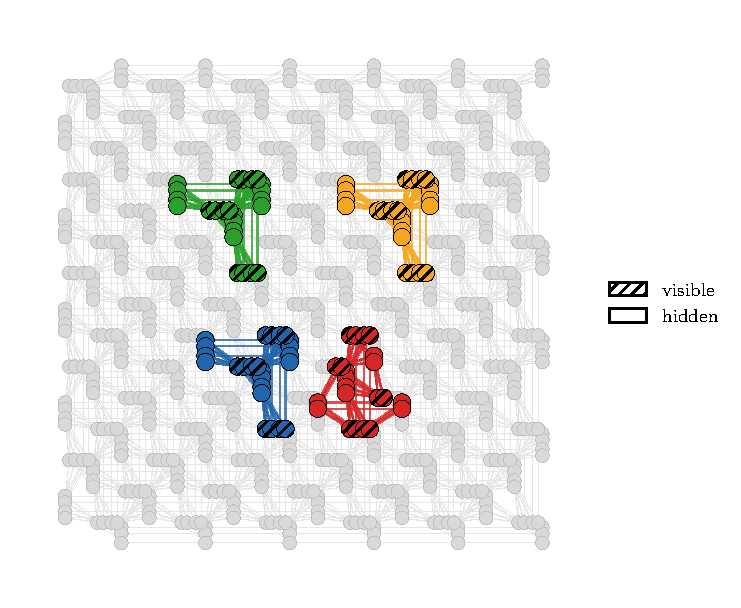
\includegraphics[width=\linewidth]{figures/parallel_embedding/parallel_embedding_np4_pegasus.pdf}}\hfill
\panel{.50}{\textbf{(b)}\\
\includegraphics[width=\linewidth]{figures/parallel_embedding/parallel_embedding_np_seeds_qpu_time.pdf}}
\caption{(a) A four-copy Pegasus embedding layout. (b) All nine recorded training trajectories vs.\ cumulative QPU access time; crosses mark divergence.}
\label{fig:parallel}
\end{figure}

\section{Marshall sign rule on the frustrated Heisenberg chain}
\label{app:marshall}

On the $N=8$ antiferromagnetic Heisenberg chain (Metropolis sampling, 200 iterations, three seeds, $J_2/J_1\in[0,1]$), fixing the Marshall sign lowers the energy error by several orders of magnitude at weak frustration, where it supplies the exact off-diagonal sign of every nearest-neighbor exchange, and the improvement shrinks as $J_2$ grows and next-neighbor exchanges (whose sign the transformation does not fix) become significant (Fig.~\ref{fig:marshall}). This is a representational result, not a sampling one: fixing $s(v)$ changes the accessible signed wavefunctions at fixed $|\psi_\theta(v)|^2$, and no improvement in sampler quality removes the restriction once frustration requires signs outside the fixed rule.

\begin{figure}[h]
\centering

\includegraphics[width=.9\linewidth]{figures/marshall_comparison/marshall_comparison_energy.pdf}
\caption{Heisenberg energy error per spin, positive-amplitude vs.\ fixed-Marshall-sign ansatz, $N=8$, three seeds. Bands are recorded standard deviations.}
\label{fig:marshall}
\end{figure}
